%\documentclass[12pt,a4paper]{report}
%\usepackage{graphicx}
%\graphicspath{ {/home/uurmi/rkwork/images/} }
%\begin{document}
\chapter{Introduction to High-performance computing}
With the advancement in technology, In recent times, Artificial intelligence(AI) has evolved, and  has changed the way we produce, manufacture and deliver. Many terms have been formulated like autonomous systems, Cognitive computing, natural language processing and machine learning. There is also a considerable advancement in the medical imaging and scientific computing fields. The common part in all these areas is that the processing data is huge, so needs more processing power than normal systems.\paragraph*{}Processing of those huge data takes significantly more time with the conventional hardware. For example, In autonomous systems to have a quicker response, the processing time should be less. And the scientific computing deals with simulations, analyses and predictions, so in this area getting quicker results saves time for the users. There are many such areas to list where quick processing of data is needed. One of the solutions to process the data in real time is increasing the processor frequency. But, the semiconductor industry is saturated with increasing the frequency of the processor and is reached a limit, beyond which the quantum effects which alter the operation of the semiconductor devices.\paragraph*{}Due to the limits in increasing frequency of operation, we have moved on to multiple processing units to process the data in parallel. This processing of large data using many computing units is coined as High-performance computing. It includes designing algorithms, methodologies, and implementations to process the data efficiently. In a single line, High-performance computing is the use of multiple processors or computers for running compute advanced applications efficiently, reliably and quickly with high throughput. Over the past few years high-performance computing has evolved considerably because of the emergence of CPU-GPU heterogeneous architectures.
% section 1.1
\section{Need for High-performance computing}
Modern CPU's are designed such that power available was plentiful and complete performance was the important figure of merit. The resulting architectures highly optimized for single-thread performance with the features such as out-of-order execution, branch prediction, and large primary instruction and data caches. In such type of designs, most of the power is used for data movement overheads, supplying the instructions and control mechanisms [5].\paragraph*{} Data movement is the central dominating area for power dissipation. The accessing time for on-chip static RAM(cache) is less than(~200 times) the time accessing DRAM. Current programming practices mainly focus on sequential, homogeneous machines with a flat view of memory, present day systems (machines) moved away from this model. With explicit control over the data movement within the memory hierarchies will result in performance sensitive code practices. Conventional architectures has a flat view of memory by having implicit data caching at multiple levels, such a practice is not sustainable for scalable systems.
\paragraph*{} The data accessing latencies in the machine will be hidden by adapting to parallel processing, especially data and fine-grained thread parallelism. A sequence of instructions is called a thread. Conventional programming systems don't provide a convenient means of providing tens of, tens of thousands of threads (or even more) on a single die. A system with such attributes is needed for parallel processsing. A system with different kinds of processors which are complement to each other in performance comprises a heterogeneous system. In a heterogeneous system, individual processors will have processing elements with different performance characteristics, different views of the memory, and will have levels of physical parallelism.

\section{Heterogeneous parallel computing}
Heterogeneous parallel computing is a hybrid word derived from two paradigms, heterogeneous computing and parallel computing. It is the processing of data in parallel using heterogeneous architecture.
\subsection{Parallel computing}
 Parallel computing is a form of computing, in which many computations are performed simultaneously. It is motivated by the fact that a large problem can be broken down into smaller ones, and all of them are solved concurrently. From the programmer’s point of view, it is mapping those parallel computations to the available compute resources.\paragraph*{}There are two aspects to consider in parallel computing; those are hardware and software.The hardware aspect is dealing with the supportive computer architecture for parallel computing. Software aspect focuses on parallel programming by fully using the computational power of the computer architecture. The parallel execution of software is possible, such that the hardware must provide a suitable platform that supports execution of multiple threads. Nowadays, processors are fabricated with a prime motivation that they should be capable of doing parallel computations. So, they are made with more than one core(multi-core). The parallel programming can be viewed as a process that maps the computation of a problem to the available cores.\paragraph*{}For sequential programming doesn’t require knowledge of the hardware architecture. But, implementing algorithms in parallel computing requires the knowledge of underlying computer architecture, in particular on the multi-core architectures.
\subsection{Types of parallelism}
 The parallel execution of an algorithm gives good utilisation of hardware and the application executes in real time. There exist mainly two types of parallelism in an application, task level parallelism and data level parallelism. The algorithm which is to be implemented using parallel computing should be analysed properly for the type of parallelism it supports.
\begin{description}
\item[Task-level parallelism] \hfill \break It is applicable if there exist many independent tasks or functions in an algorithm. For example, if there are three tasks in an application such as decoding video, processing video, and displaying the output. Even though each task has dependency with each other, they can be made independent by executing them using a three stage pipeline on different cores. We have used this methodology in implementing computer vision algorithms on a Rcar-H3 SoC which has an active quad-core ARM A-57.
\item [Data parallelism] \hfill \break  On the other hand, Data parallelism is possible when there exist many data elements that can be operated independently. It focuses mainly on distributing data elements to multiple threads on multiple cores. This Data level parallelism is most useful in heterogeneous programming where the hardware contains a complementary coprocessor which is capable of handling the execution of multiple data elements at once. We followed CUDA programming to address the data parallel portions in the algorithms.
\end{description}
\subsection{Classifications of Computer architecture}
%bullets
According to Flynn’s Taxonomy\cite{flynn} there exist four types of computer architectures,
\begin{enumerate} 
\item Single Instruction Single Data (SISD) \hfill
	\begin{itemize} 
	\item Traditional computer architecture is a serial architecture. They use unicore processors, only one instruction stream is executed in a cycle.
	\end{itemize}
\item Single Instruction Multiple Data (SIMD)
\begin{itemize} 
\item These type of computers use multi core processors, all the cores execute the same instruction stream but operates on different data streams. This architecture is used extensively in this work.
\end{itemize}
\item Multiple Instruction Single Data (MISD)
\begin{itemize} 
\item This architecture is very rarely used where separate instruction streams will operate on same data streams.
\end{itemize}
\item Multiple Instruction Multiple Data (MIMD)
\begin{itemize} 
\item In this architecture different instruction streams works on different data.
\end{itemize}
\end{enumerate}
\noindent Recently the computer architecture is moving from muti-core to many-core, many-core means having a high number of cores(tens or hundreds). For example a GPU represents a many core architecture, and it supports every type of parallelism we have described previously such as SI MD, MIMD,multi-threading and Instruction level parallelism (ILP). This type of architectures are called Single instruction multiple threading(SIMT). Recently GPUs have been evolved to be more powerful  with SIMT architecture. So, they tackle the massively parallel computations, and they are fully programmable for general purpose computing.
\subsection{Heterogeneous computing}
Heterogeneous computing refers to systems that use multiple types of processors. These are multi-core systems that gain performance not only by adding cores but also by incorporating special processing capabilities to specific tasks. Heterogeneous System Architecture (HSA) systems use multiple types of processors (typically CPUs and GPUs), usually on the same silicon chip or added discretely to the central processor. GPU processing, aside from the well-known 3D graphics rendering, can be used for Mathematically intensive calculations on vast amounts of data, while CPUs can run the operating system and perform traditional serial tasks.\paragraph*{}This is the reason the heterogeneous computing that brings the best of both CPUs and GPUs is essential to drive faster and more powerful processor designs for new and better experiences. GPU is added to a system as a coprocessor to CPU, which supplements its functionalities for the tasks where CPU overloads. This brings a new world of computing where the compute and bandwidth intensive tasks offload the CPU, and the CPU continues it's sequential execution smoothly.
\subsection{Heterogeneous architecture}
GPU currently is not a standalone platform, but it is attached to CPU as a coprocessor through a PCI-Express bus so that it will work in conjunction with CPU. The CPU monitors all the GPU activities. CPU is called a host and GPU a device. The Figure \ref{Figure:1.1} shows the CPU-GPU environment.
\begin{figure}[h!]
  \centering
  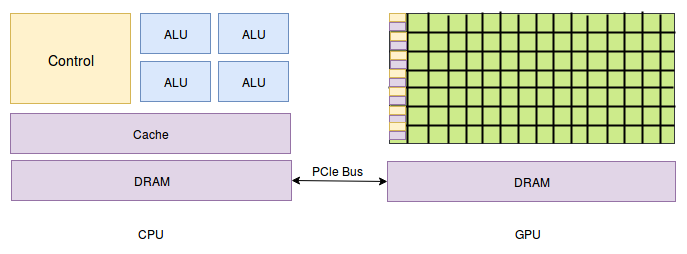
\includegraphics[width=0.8\linewidth]{HeteroGeneousArch.png}
  \caption{Heterogeneous architecture}
  \label{Figure:1.1}
\end{figure}
In a heterogeneous application, there are two types of codes, a host code that runs on CPU and a device code that runs on GPU. Allocating suitable portions of code for CPU and GPU makes the application perform in real time. CPU initializes the heterogeneous application and will manage environment, data and code to the device. CPU-GPU heterogeneous parallel computing architectures are introduced because the CPU and GPU have complementary attributes and that enable applications to run efficiently using both types of processors. So the sequential parts of the application execute on the CPU and the intensive data parallel parts run on the GPU as shown in the Figure \ref{Figure 1.2}. The NVIDIA GPUs are used in this work to maintain a heterogeneous architecture.
\begin{figure}[h!]
  \centering
  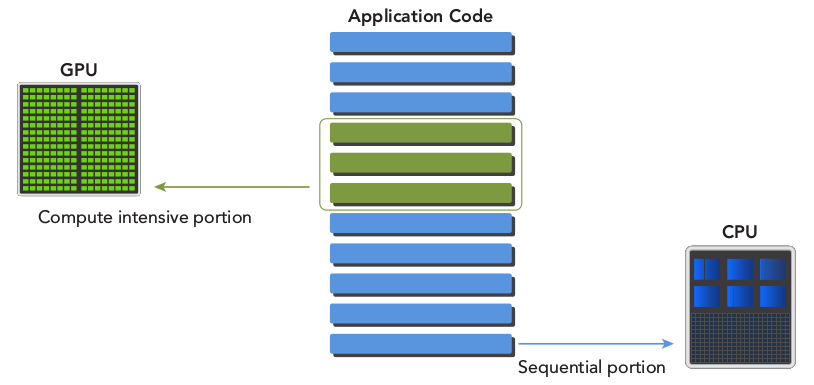
\includegraphics[width=0.75\linewidth]{seq-parallel.png}
  \caption{Distributing the Heterogeneous code to the suitable processor}
  \label{Figure 1.2}
\end{figure}
\paragraph*{} In the heterogeneous architecture the GPU may be integrated into the processor or added externally to the CPU. The discrete GPUs are more common than integrated in the case of desktop PCs. where as in the mobile computing platform integrated GPUs are quiet common. For this work a desktop PC with NVIDIA GPU is used. NVIDIA GPU is preferred for this work because of its ease of programming. A term is coined for using GPU for general purpose programming, which is GPGPU(General purpose programming on Graphics Processing Unit). GPGPU is supported through frameworks such as OpenCL,CUDA etc. Compute Unified Device Architecture (CUDA) is predominant now a days because of its simple and efficient APIs, it is used to program NVIDIA GPUs. The following product families of NVIDIA exhibit the GPU computing platform.
\begin{enumerate} 
\item \textbf{GeForce} \hfill \break It is designed especially for consumer graphics.
\item \textbf{Quadro} \hfill \break This product family is suitable for professional visualization.
\item \textbf{Tesla} \hfill \break This family of products mainly used for parallel computing at data center .
\item \textbf{Tegra} \hfill \break It is designed specially for mobile and embedded computing platforms.
\end{enumerate}
NVIDIA GPUs are classified within the product family according to their architectures such as Fermi,Kepler, Maxwell and Pascal. Each architecture has their own benefits from the previous architectures. In this work Kepler architecture NVIDIA GPU is used. The selection of suitable GPU platform is based upon the following important features.

\begin{itemize}
\item Number of GPU cores
\item Memory size
\end{itemize}

\section{NVIDIA GPU architecture}
As shown in the Figure \ref{Figure:1.3}, the NVIDIA GPU contains an array of streaming multiprocessors (SM), each SM is capable of running thousands of concurrent threads. The SM in the GPU is a set of processors. A thread is a sequence of instructions to be executed on a processor. A group of threads are called a warp, each warp executes per each instruction cycle in an SM. Instruction level parallelism is extracted by pipe-lining the instructions in each thread. There is no branch prediction and speculative execution in GPU. NVIDIA GPUs use different types of memory for performance improvements in the Data movement. The shared memory used is local to the block of threads and has very less memory transaction cost. The texture and constant memories are useful for special type of applications and will move the data very fast.
\begin{figure}[htb]
	\centering
	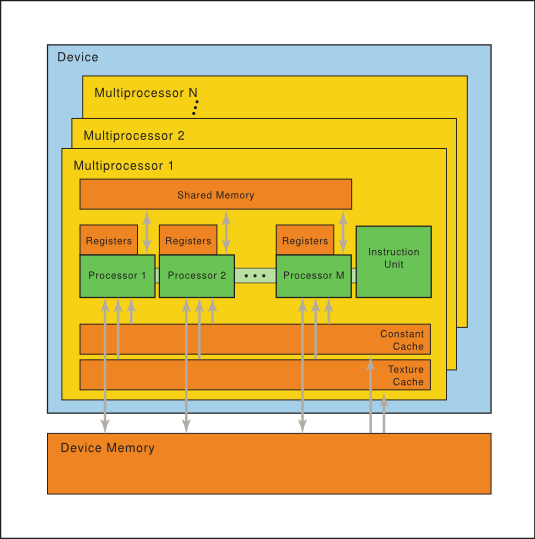
\includegraphics[width=0.8\linewidth]{hardware-model.png}
	\caption{NVIDIA GPU hardware model}
	\label{Figure:1.3}
\end{figure}
\paragraph*{}By Using CUDA platform one can access all the NVIDIA GPU features explained above. CUDA is becoming more significant now a days because of its simple interfaces, and is evolved as a Heterogeneous computing platform that enables the users to easily write heterogeneous programs onto NVIDIA GPU’s.